\documentclass[10pt,a4paper]{article}
\usepackage[utf8]{inputenc}
\usepackage[T1]{fontenc}
\usepackage{lmodern}
\usepackage[margin=1.5cm, top=1.4cm, bottom=1.4cm]{geometry}
\usepackage{hyperref}
\usepackage{enumitem}
\usepackage{titlesec}
\usepackage{xcolor}
\usepackage{graphicx}

\definecolor{accent}{HTML}{00686E}
\hypersetup{colorlinks=true, urlcolor=accent, linkcolor=accent}
\pagenumbering{arabic}
\setlength{\parindent}{0pt}

\titleformat{\section}{\large\bfseries\color{accent}}{}{0em}{}[\vspace{-0.6em}\rule{\textwidth}{0.8pt}]
\titlespacing{\section}{0pt}{7pt}{4pt}

\newcommand{\role}[4]{%
  \textbf{#1} \hfill \textbf{#2}\\[1pt]%
  \textit{#3} \hfill \textit{#4}\\[2pt]%
}
\setlist[itemize]{leftmargin=1.2em, itemsep=1.5pt, topsep=2pt, parsep=0pt}

\begin{document}

% ================= HEADER =================
\begin{minipage}[c]{0.80\textwidth}
  {\Huge\bfseries Prabhavit Gupta}\\[3pt]
  {\color{accent}\large Cloud \& AI Engineer: Python APIs, RAG Architectures \& LLM Systems}\\[6pt]
  {\footnotesize +39 351 610 7807 ~$\vert$~
  \href{mailto:prabhavitg@gmail.com}{prabhavitg@gmail.com} ~$\vert$~
  \href{https://www.linkedin.com/in/prabhavit/}{linkedin.com/in/prabhavit} ~$\vert$~
  \href{https://github.com/prab-gupta}{github.com/prab-gupta} ~$\vert$~
  Venice, Italy (Resident in Italy / Permesso di Soggiorno UE a Tempo Indeterminato)}
\end{minipage}\hfill
\begin{minipage}[c]{0.18\textwidth}
  \raggedleft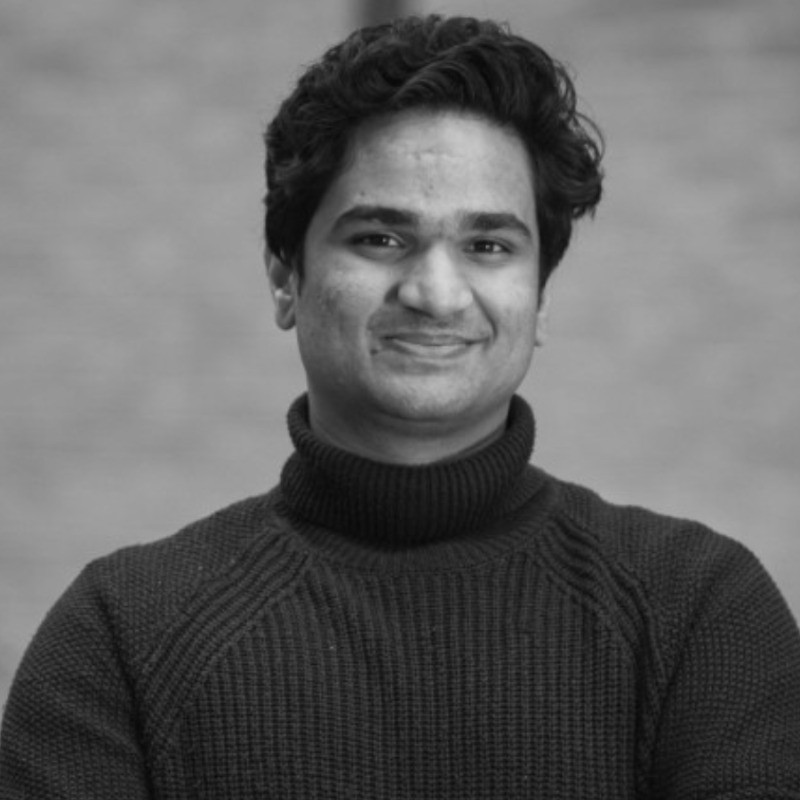
\includegraphics[width=2.0cm]{photo.jpg}
\end{minipage}
\vspace{-2pt}

% ================= SUMMARY =================
\section{Summary}
Cloud and AI Engineer with 3 years of production software engineering experience architecting scalable Python APIs, Retrieval-Augmented Generation (RAG) architectures, and cloud-integrated LLM systems. Hands-on expertise developing production frameworks with FastAPI, LangChain, vector retrieval pipelines, and asynchronous messaging systems. Resident in Venice, Italy with an EU Long-Term Residence Permit (permanent unrestricted Italian and EU work authorization, no sponsorship required). Bilingual English (C1 Professional), Italian (conversational/parlato); available immediately for full-time cloud and AI engineering roles.

% ================= TECHNICAL EXPERTISE =================
\section{Technical Expertise}
\begin{itemize}
  \item \textbf{AI Engineering \& LLM Systems:} Architetture RAG, LangChain, OpenAI / Claude API integration, vector embeddings, semantic search, hybrid retrieval, prompt engineering, agentic function calling.
  \item \textbf{Cloud Infrastructure \& Orchestration:} Cloud engineering, Docker containerization, asynchronous messaging (Pub/Sub, Redis queues), RESTful API design, CI/CD pipeline automation, GitOps.
  \item \textbf{Backend Development \& Python:} Python (FastAPI, asyncio, pandas, NumPy, Pydantic), TypeScript, Node.js, microservices architecture, JSON schema enforcement, database modeling.
  \item \textbf{Databases \& Data Management:} PostgreSQL (relational modeling, indexing, query optimization), Redis caching, vector stores, data extraction and ETL transformation pipelines.
  \item \textbf{Testing \& Observability:} End-to-end integration testing with Playwright, API contract verification, cloud monitoring, structured logging, latency and cost optimization.
  \item \textbf{Languages \& Authorization:} Italian (Parlato/Conversational), English (C1 Professional, fluent), Hindi (Madrelingua). Permesso di Soggiorno UE a tempo indeterminato (autorizzazione illimitata al lavoro in Italia e UE).
\end{itemize}

% ================= EXPERIENCE =================
\section{Experience}

\role{\href{https://flowspace.co}{FlowSpace.co}}{Mar 2024 - Aug 2026}{Lead Developer \& AI Systems Architect}{London, UK (remote)}
\begin{itemize}
  \item Engineered production cloud AI services and RAG search pipelines for a marketplace platform serving 4,500+ active enterprise users across Europe.
  \item Developed high-throughput Python (FastAPI) and Node.js backend APIs, integrating vector retrieval and LLMs with internal PostgreSQL databases.
  \item Built LangChain orchestration workflows with automated context injection and tool execution, reducing edge-case query failure rates.
  \item Implemented semantic caching and asynchronous task processing using Redis and message queues, optimizing cloud resource consumption and query latency.
  \item Deployed Docker containers across cloud infrastructure with automated CI/CD deployment pipelines and comprehensive API contract testing.
  \item Managed monitoring, distributed logging, and incident response for AI API microservices, maintaining high operational availability.
\end{itemize}

\role{Urlink}{Apr 2025 - Jul 2025}{Project Manager \& Solutions Developer (Freelance)}{Barcelona, Spain (remote)}
\begin{itemize}
  \item Led technical discovery, solution architecture, and delivery of cloud-integrated web services and data processing pipelines for European clients.
  \item Built automated ETL data ingestion services connecting external APIs to relational databases, ensuring consistent data synchronization.
  \item Developed interactive prototypes to validate API specifications and architecture designs prior to production deployment.
\end{itemize}

\role{Independent Technical Consultant}{Aug 2023 - Feb 2024}{AI Automation \& Integration Developer}{Venice, Italy}
\begin{itemize}
  \item Designed and deployed custom Python automation microservices, webhook listeners, and LLM integrations for SMB clients in Italy and Europe.
  \item Automated document processing and structured data extraction workflows, replacing fragile manual data entry with resilient event-driven systems.
  \item Authored technical architecture documentation, API guides, and system configuration manuals for client engineering teams.
\end{itemize}

% ================= EDUCATION =================
\section{Education}
\role{Ca' Foscari University of Venice}{2020 - 2024}{BA in Philosophy, International Studies and Economics}{Venice, Italy}
\begin{itemize}
  \item Rigorous training in formal logic, analytical problem solving, systems analysis, and macroeconomic decision models.
\end{itemize}

\end{document}
